\documentclass{letter}
\usepackage[top=0.5cm, bottom=0.5cm]{geometry}
\usepackage{hyperref}
\usepackage{graphicx}
\usepackage{wrapfig}

%\usepackage{lipsum}

\address{\\ \\ \\ \large \textbf{Branch of} \\ \large \textbf{
Oral and Maxillofacial Surgery} \\ Wan-Fang Hospital,\\ Taipei Medical University \\}
\date{}

\begin{document}
\begin{letter}
{
\centering \Large \textbf{Letter of Recommendation}
}

\hfill
\begin{wrapfigure}[1]{l}{0.65\linewidth}%{height=0.65\textheight}
    %\centering
    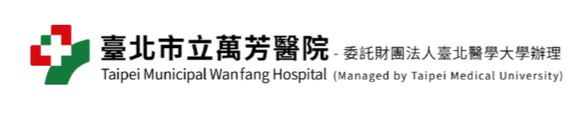
\includegraphics[width=0.3\textheight]{TMWH.png}
\end{wrapfigure}

\opening{To Whom it May Concern:} % admissions officer
\medskip 

Dr. Sun Yihua, a talented and intelligent doctor, is deeply interested in oral and maxillofacial surgery during her PGY training, and take it as her mission to become a "real doctor". 
With 3.5 years of specialty training in oral and maxillofacial surgery, she is tenacious, interactive, and tireless. 
She rounds the ward on time every day of the year, 24 hours a day, 365 days a year, guards patients, and follows the attending physician's directions. Even though she had a cold, she was invigorated to undergo oral cancer surgery the next morning after obtaining an intravenous injection in the ward.
When the COVID-19 epidemic breaks out in Taiwan in 2021, despite her family's concerns, she will remain at her post and aid the oral and maxillofacial surgery in the crisis.

It is recommended that Dr. Sun meet the conditions and be nominated as Professor Yin Niande's Outstanding Rookie Award, which is well-deserved, and hope that in her career as a specialist, she will continue to follow her original intention and serve the welfare of patients.

\medskip
Sincerely, \\
Chi, Li-Hsing Tex \\
Director of OMS, TMWH

\end{letter}
\end{document}